In this chapter, we build a complete picture of the Methodology applied during the subject research. We briefly analyze the dataset used and describe all components of the implemented model and the training script used to generate the optimal weights for these components.

\section{Data Analysis and Exploration} \label{sec:data_analysis}

The dataset selected for sourcing the prediction model was part of the NeurIPS2021 Traffic4cast competition \cite{pmlr-v176-eichenberger22a}. This dataset consists of 360 days of data from 8 different cities with similar sizes derived from trajectories of a fleet of probe vehicles. The original data has 180 days from 2019 and another 180 days from 2020, as one of the questions of the challenge was to asses how the COVID pandemic affected traffic in different cities. As this represents a shift in the temporal distribution of the data, we choose not to use the 2020 half of it, intending to have an assumed temporal invariant distribution. Table\ref{tab:cities} disposes of all cities available on the dataset and the number of data points each city contains.

\begin{table}[!ht]
\centering
\begin{tabularx}{\textwidth}{ M | M | M }
\multicolumn{1}{X}{\textbf{City}}%
& \multicolumn{1}{X}{\textbf{\# of days}} 
& \multicolumn{1}{X}{\textbf{\# snapshots per day}}\\ \hline
Antwerp & 180 & 240 \\ \hline
Bangkok & 180 & 240 \\ \hline
Barcelona & 180 & 240 \\ \hline
Berlin & 180 & 240 \\ \hline
Chicago & 180 & 240 \\ \hline
Istanbul & 180 & 240 \\ \hline
Melbourne & 180 & 240 \\ \hline
Moscow & 180 & 240 
\end{tabularx}
\caption{List of the cities available on the dataset}
\label{tab:cities}
\end{table}

For a given time snapshot, the data of one city can be represented by a tensor of size $(495, 436, 8)$, where $495\times436$ represents the city grid, and $8$ stands for the channels, or pieces of information, per cell. These channels contain information on the volume and mean speed of the probe cars heading in the four diagonal directions. All data was normalized and discretized in the \texttt{uint8} range, meaning values are contained in the $[0, 255]$ range.

To better understand the data, distribution, and characteristics, the following analysis is conducted on the 5-minute snapshot that started at 12:00 on 9 January 2019 in Melbourne. Figures \ref{fig:speed} and \ref{fig:volume} show the distribution of values for both the speed (odd channels) and the volume (even channels). It's clear that while the volume has a more even distribution for non-zero values, there remains a massive bias for the zero values, as they represent more than 99\% of the data points. This indicates that most of our data comprises zeros and that activity should be treated as rare.

Furthermore, Figure \ref{fig:heatmap} confirms this theory, as it can be seen that most of the data for the speed channels is zero, and the volume, despite being better distributed, is also defined by a majority of zeros. Table \ref{tab:data_analysis} shows the statistics for each channel and reinforces the proposed thesis.



\begin{figure}[!ht]
    \centering
    \begin{minipage}{0.45\textwidth}
        \centering
        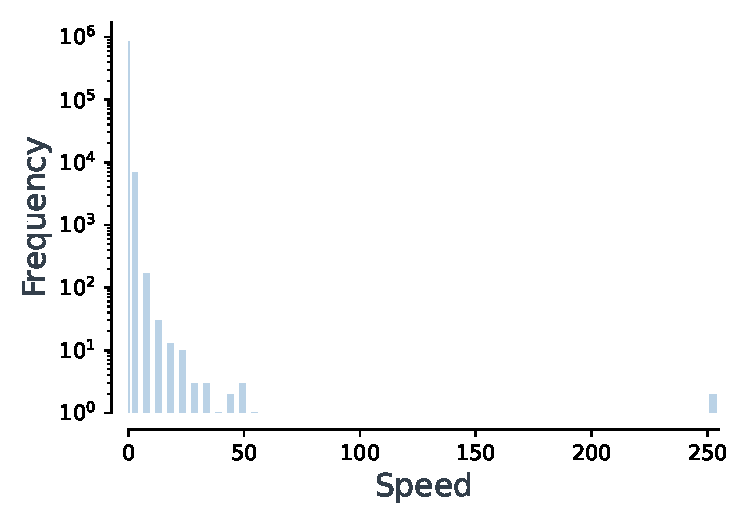
\includegraphics[width=0.9\textwidth]{./figures/speed.pdf}
         \caption{Histogram for data distribution for the speed. Note the first (very thin) bin with the null values.}
         \label{fig:speed}
    \end{minipage}\hfill
    \begin{minipage}{0.45\textwidth}
        \centering
        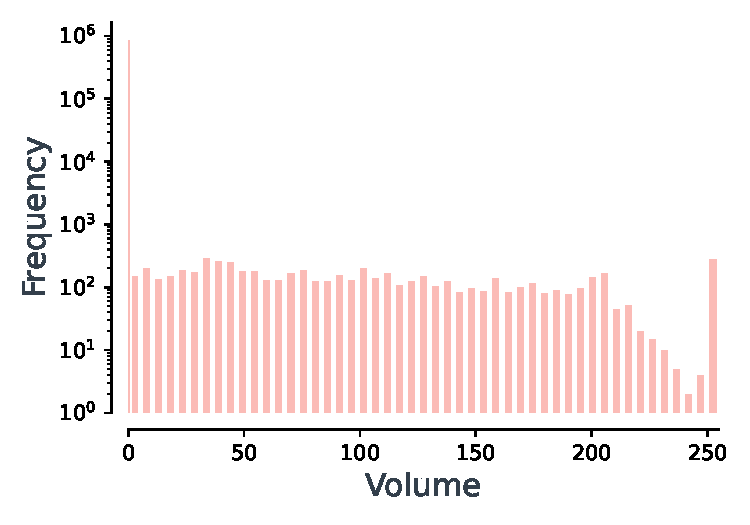
\includegraphics[width=0.9\textwidth]{./figures/volume.pdf}
         \caption{Histogram for data distribution for the volume. Note the first (very thin) bin with the null values.}
         \label{fig:volume}
    \end{minipage}
\end{figure}


\begin{figure}[!ht]
\noindent\hspace{0.5mm}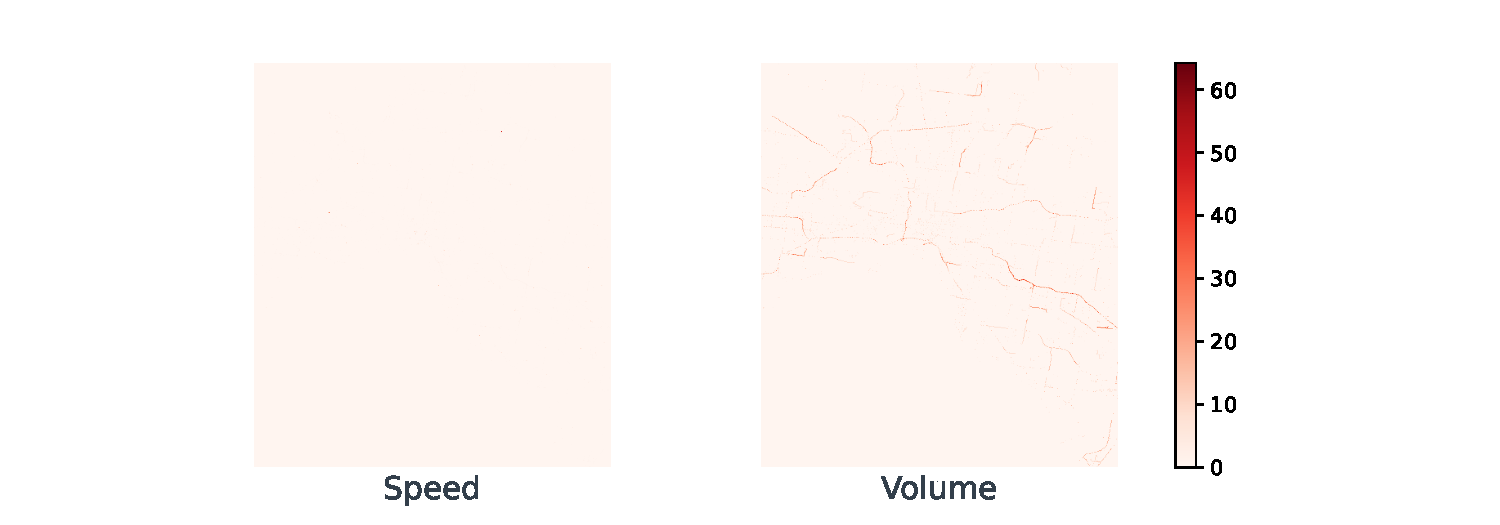
\includegraphics[width=0.9\textwidth]{./figures/heatmaps_speed_volume.pdf}
\caption{Heatmap of the snapshot for the (a) Speed; and (b) Volume.}
\label{fig:heatmap}
\end{figure}


\begin{table}[!ht]
\centering
\begin{tabularx}{\textwidth}{ M | M | M | M | M }
\multicolumn{1}{X}{\textbf{Channel}}%
& \multicolumn{1}{X}{\textbf{Mean}} 
& \multicolumn{1}{X}{\textbf{Median}}
&\multicolumn{1}{X}{\textbf{Standard Deviation}}
&\multicolumn{1}{X}{\textbf{Non-zero elements}} \\ \hline
0 (volume) & 0.0216 & 0.0000 & 0.2861 & 1.08\% \\ \hline
2 (volume) & 0.0141 & 0.0000 & 0.2794 & 0.84\% \\ \hline
4 (volume) & 0.0133 & 0.0000 & 0.6236 & 0.72\% \\ \hline
6 (volume) & 0.0118 & 0.0000 & 0.5957 & 0.62\% \\ \hline
1 (speed)  & 0.6758 & 0.0000 & 9.5058 & 0.73\% \\ \hline
3 (speed)  & 0.8655 & 0.0000 & 11.3655 & 0.82\% \\ \hline
5 (speed)  & 0.7419 & 0.0000 & 10.5863 & 0.71\% \\ \hline
7 (speed)  & 0.6149 & 0.0000 & 9.8281 & 0.60\%
\end{tabularx}%
\caption{Statistics for each channel in the specific snapshot}
\label{tab:data_analysis}
\end{table}

\subsection{Data processing}

Some other data processing transformations were processed besides disposing of the 2020 half of the original data. A significant part of the motivation for this processing step is to reduce the input data's size (or shape) to make the models trainable in a reasonable time, given the limited computational resources available. The first one of the transformations implemented was the collapse of the even (volume) and odd (speed) channels by taking the mean of the data in every channel. Therefore, we were left with two channels: the volume and average speed of the cars in the particular region.


Furthermore, to allow efficient development of the model's components, only the central square of size $50\times 50$ was employed for the preliminary tests and experiments, including those used to tune the model's parameters. This may seem limiting at first glance, as it reduces the spatial coverage and may exclude potentially significant peripheral data. Nonetheless, this strategy is practically beneficial as it simplifies computational demands while capturing a substantial portion of traffic behaviors. The selected central area includes key urban sections characterized by informative traffic dynamics, which will help scale the model to encompass the entire urban layout.


%\begin{figure}[!ht]
%\noindent\hspace{0.5mm}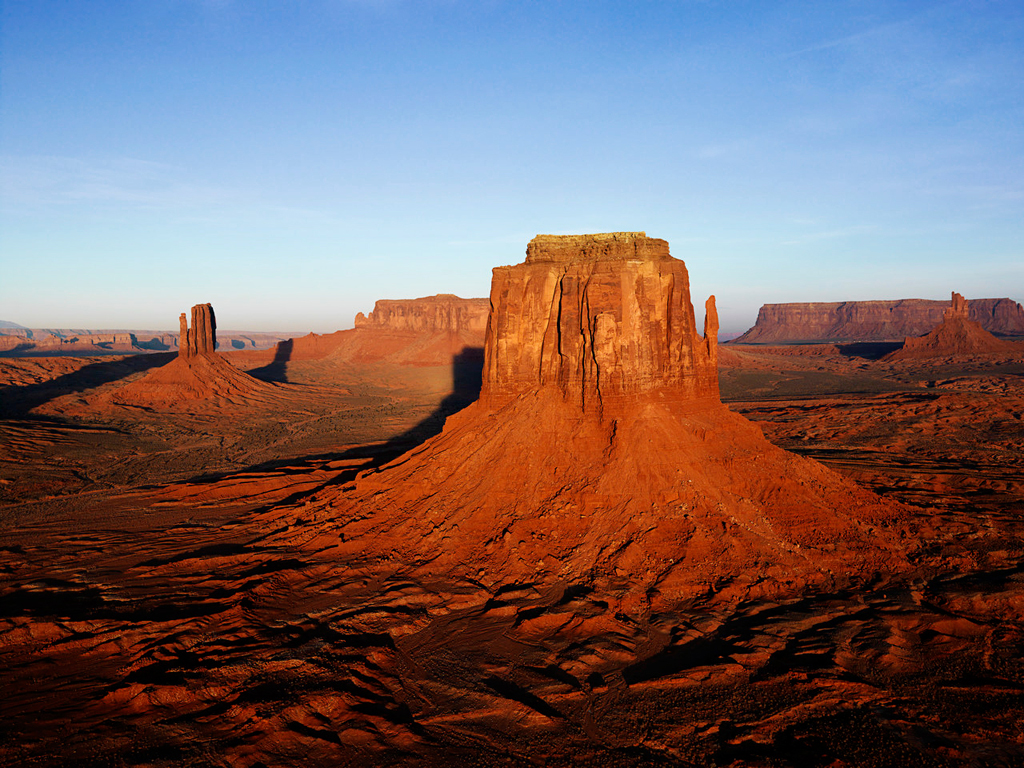
\includegraphics[width=12cm]{./resources/Desert.jpg}
%\caption{Title, Author}
%\end{figure}


\section{Model Outline}

The proposed model consists of two modules: a Feature Extraction Network, modeled as the encoder of an autoencoder and explained in Section \ref{sec:fen}, and a Prediction Network, thoughtfully dissected in Section \ref{sec:pred}. Furthermore, Section \ref{sec:domainadap} is reserved for the exposition of the domain adaptation techniques employed through the model and during training to enable knowledge transfer between the domains. Section \ref{sec:training} summarizes with figures and pseudocode scripts how the model's training was done. This Section will explain the mathematical and formal basis for the model and the overall architecture to be built.


\todo[inline]{double check sections}

\subsection{Task}
The field of Spatio-Temporal prediction is vast, allowing researchers to try different approaches to problems that may seem the same. This can be observed from the bibliography presented in the bibliographic revision. It's essential to clearly define the problem to be solved and rigorously define the available information.

\begin{definition}\label{def:part}
A city $C$ is divided into a grid map of shape $W_{C}\times H_{C}$. Each partition $r_{i, j}$, with $1\leq i \leq W_C$ and $1\leq j \leq H_C$, is referred to as a region of $C$. The set containing all regions of the city is defined $R_C=\{r_{1, 1}, ..., r_{W_C, H_C}\}$.
\end{definition}

\begin{definition}\label{def:time}
The time range of available data of a city is divided into $T_{C}$  intervals of equal size: $t=[1, ..., t_{C}]$.
\end{definition}


\begin{definition}\label{def:ch}
For each region $r_{i, j}$, $N_{ch}$ data channels are available. These channels are the same for every city.
\end{definition}

By combining Definitions \ref{def:part}, \ref{def:time}, and \ref{def:ch} we can visualize the the 4D tensor of shape $(W_C, H_C, N_{ch}, T_C)$. Figure \ref{fig:data_tensor} shows a slice of this tensor. Each color represents a different channel, and each square of four colors represents a point in the 2D city grid. The stacked layers represent the time dimension.

\begin{definition} \label{def:dim}
A 4D tensor defines the data of a city $C$:
	\begin{equation}\label{eq:defdim}
		\mathcal{X}_C = \{x_{r, t}^{ch} | r \in R_C, t \in T_c, ch \in N_{ch}\}
	\end{equation}
\end{definition}

\begin{figure}[!ht]
\noindent\hspace{0.5mm}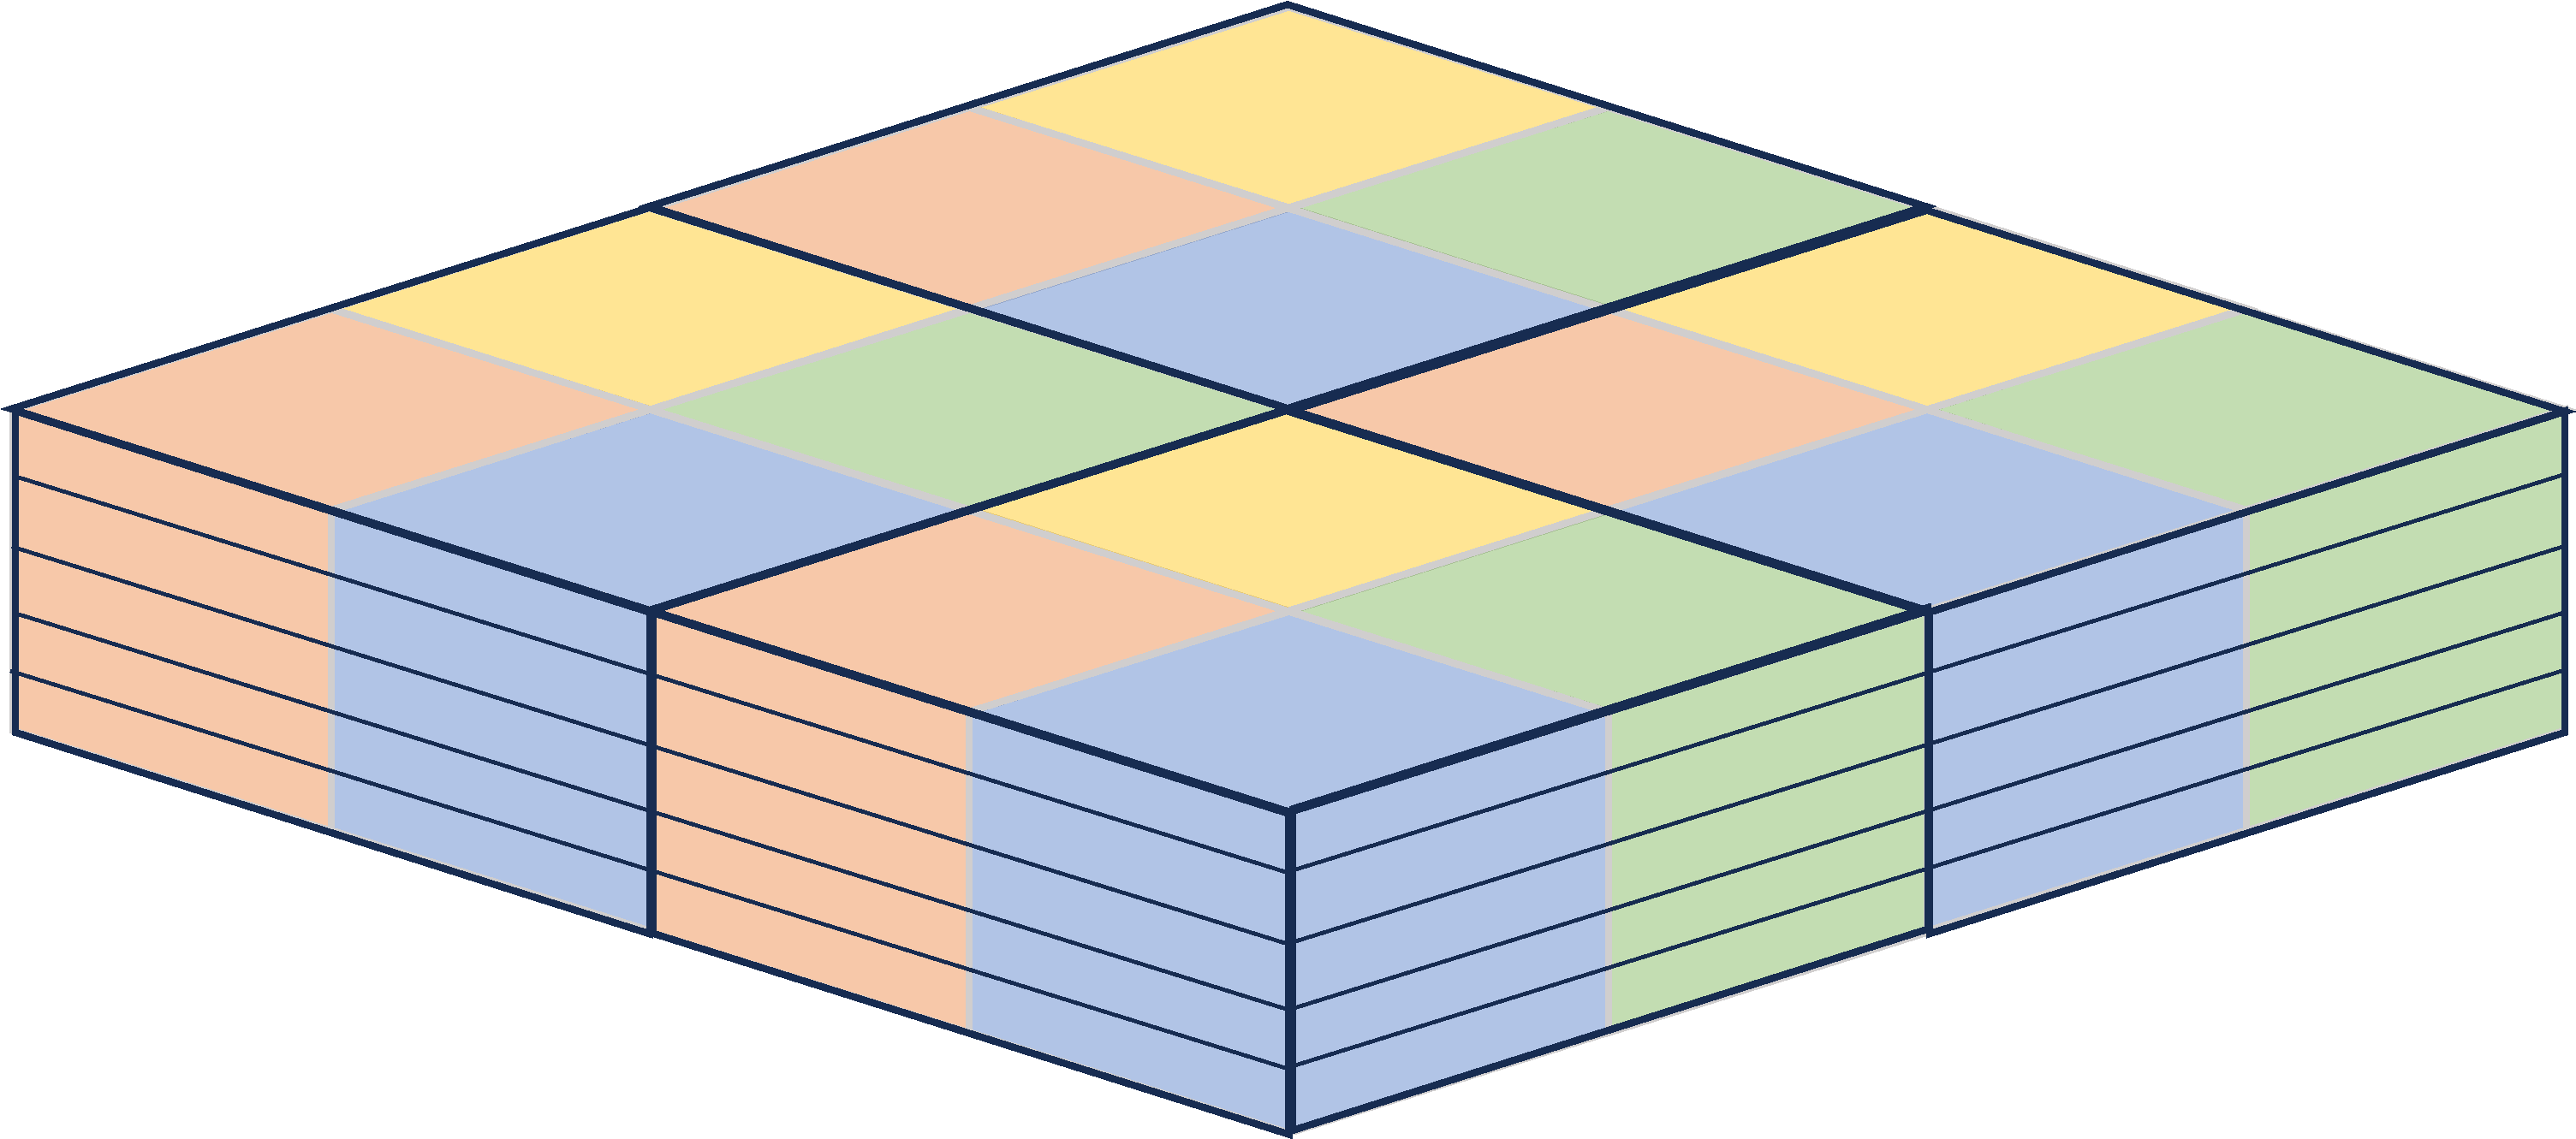
\includegraphics[width=0.6\textwidth]{./figures/data_tensor.pdf}
\caption{Visualization of the data (as a tensor).}
\label{fig:data_tensor}
\end{figure}

\begin{definition}\label{def:conn}
Connectivity in the city grid, denoted as \( \mathcal{E}_C \), is defined by the set of edges that establish the relationship between adjacent regions in \( C \). Each edge \( e_{k,l} \) in \( \mathcal{E}_C \) connects two regions \( r_{i,j} \) and \( r_{m,n} \), where \( i \) and \( m \) are indices within the width of the grid \( W_C \) and \( j \) and \( n \) are indices within the height of the grid \( H_C \). An edge exists if the regions it connects are adjacent horizontally, vertically, or diagonally, allowing for traffic data flow and convolutional operations across regions. Formally, the connectivity is represented as:
$$
\begin{aligned}
\mathcal{E}_C = \{ & e_{k,l} | e_{k,l} \text{ connects } r_{i,j} \text{ and } r_{m,n}, \text{ such that } |i - m| \leq 1 \text{ and } |j - n| \leq 1, \\
& \text{ for all } i, j, m, n \text{ that satisfy } 1 \leq i, m\leq W_C \text{ and } 1 \leq j, n \leq H_C \}
\end{aligned}
$$
\end{definition}


\begin{definition}\label{def:graph}
A graph representation of a city \( C \), denoted as \( G_C \), is defined as a tuple \( (V_C, \mathcal{E}_C,\mathcal{X}_C) \), where \( V_C \) is the set of nodes corresponding to the regions of \( C \), \( \mathcal{E}_C \) is the set of edges representing connectivity between regions, and \(\mathcal{X}_C \) is the node feature matrix, containing the feature (or channel) values of each node in \( V_C \). 
\end{definition}

Putting all previous definitions together, we define the adjacency matrix:

\begin{definition}\label{def:adj_matrix}
The adjacency matrix for a city \( C \), denoted as \( \mathbf{A}_C \), is a matrix that represents the connectivity between the nodes of \( C \) as defined in \( \mathcal{E}_C \) from Definition \ref{def:conn}. The adjacency matrix is a square matrix of size \( |V_C| \times |V_C| \), where \( |V_C| \) is the number of nodes in the graph representation of the city. Each element \( a_{ij} \) of the matrix \( \mathbf{A}_C \) is defined as follows:

$$
a_{ij} = 
\begin{cases}
1, & \text{if there exists an edge } e_{ij} \in \mathcal{E}_C \text{ connecting nodes } v_i \text{ and } v_j \\
0, & \text{otherwise}
\end{cases}
$$

This matrix is symmetrical, as the presence of an edge \( e_{ij} \) implies bidirectional connectivity between the nodes \( v_i \) and \( v_j \).
\end{definition}



With these definitions, it's possible then to define Problem \ref{prob:tl}:

\begin{problem} \label{prob:tl}
Given a data-scarce target city, $C_T$, and a set of $n$ data-rich source cities $\{C_{S1}, ..., C_{Sn}\}$, the problem proposed is to predict the value of the target city's data at $t_T+1$ with the historical data of the target city itself to that point and of the source cities:
	\begin{equation}\label{eq:probtl}
		\min_{\theta}\mathcal{L}(\tilde{\mathcal{X}}_{T, t_T + 1}, \mathcal{X}_{T, t_T + 1} )
	\end{equation}
	where
	\begin{equation}\label{eq:probtl2}
		\tilde{\mathcal{X}}_{T, t_T + 1} =  \theta(\mathcal{X}_{T, 1:t_T}, \{\mathcal{X}_{S1}, ..., \mathcal{X}_{Sn}\})
	\end{equation}
\end{problem}

Note that $ \mathcal{L}$ is the error criterion, which may vary depending on the data requirements. Note also that $t_{Sk} \gg t_T \forall k=1, ..., n$, indicating the target city's scarcity and the sources' richness.

\subsection{Proposed Architecture}

As explained at the beginning of this Section, the model comprises a Feature Extractor block modeled after the encoder of an autoencoder and a Predictor block. Figure \ref{fig:network_simplified} outlines the proposed architecture. Note that the individual modules will be developed and explained in their sections. The architecture adopted in this research draws upon the works of \cite{Wang202222, Wang20224695} as they proposed similar divisions in their models to transfer knowledge. Compared to their approach, we suggest using a \gls{STGAE} to train the feature extractor and an adjacency matrix to represent connectivity between the regions. Furthermore, the training part of the presented model is influenced by the work of \cite{Tang2022}, as we use similar domain adaptation techniques but delve into the influences that diversity on the source domain exerts on the model's accuracy.

\begin{figure}[!ht]
\noindent\hspace{0.5mm}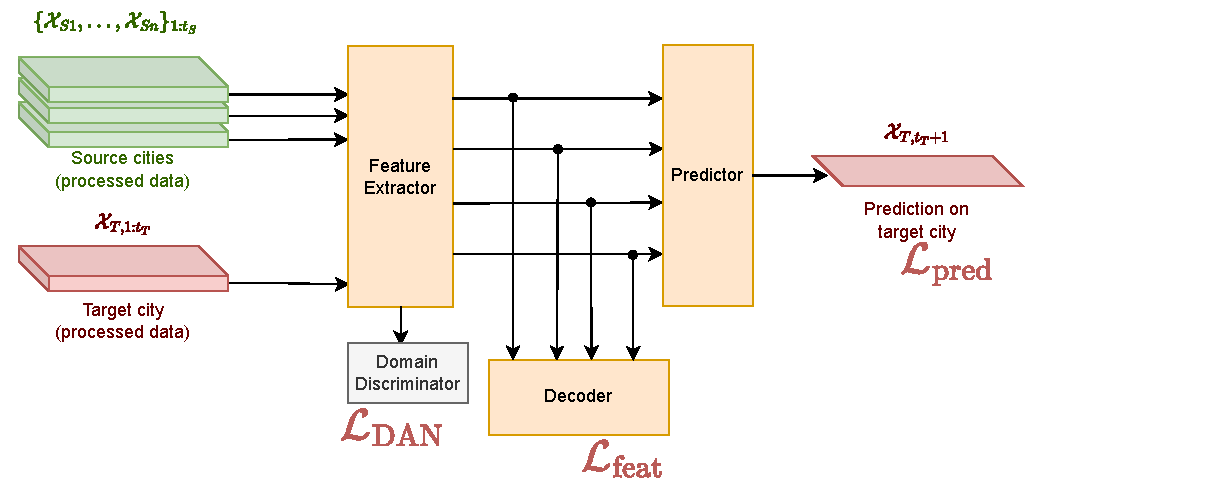
\includegraphics[width=0.9\textwidth]{./figures/Model.pdf}
\caption{Simplified version of the proposed model.}
\label{fig:network_simplified}
\end{figure}

\section{Feature Extraction Network} \label{sec:fen}

As the first layer of the model, the Feature Extraction Network receives an input of tensors from one or more source cities and the target city and tries to extract, from these tensors, \gls{ST} features must be extracted to be used to train the Prediction Network. 

\subsection{Autoencoder}
 
Selecting hyperparameters and fine-tuning an extractor are challenging tasks in constructing a model, as it's difficult to observe causality between the change of a parameter and the change of the output due to the highly non-linear characteristics of these modules. As a result of these problems, the use of autoencoders for the feature extraction task has been proposed by \cite{Hinton2006}, and it's, as of today, a well-established paradigm in the \gls{ST} field. By conceptualizing the feature extraction process through the lens of an encoder, it becomes easier to verify its quality by constructing a corresponding decoder. As the encoder maps the input data from its original vectorial space to a latent space, the decoder pursues the contrary operation, returning the data from the latent space to the original one. In an ideal scenario, a well-trained autoencoder will reconstruct the original data perfectly, guaranteeing the quality of the features extracted by the encoder.
 
More recently, \cite{fan2023spatiotemporal} implemented a \gls{STAE} by coupling \gls{GLU} layers for time convolution and Chebyshev convolution layers for spatial convolution. By interpolating two temporal layers by a spatial one, the authors extracted both spatial and temporal features. Additionally, using Chebyshev filters of relatively large sizes ($K=6$), the proposed autoencoder could correctly derive features on both local and global scales.

In another paper, \cite{sabbaqi2022graph} proposes a generic framework for \gls{STGAE} with symmetric encoder-decoder architectures. The encoder finds a latent graph representation by applying graph convolutions, temporal downsampling layers, and activation functions. The decoder mirrors this behavior but uses temporal upsampling layers between the convolutions and activation functions. 
 
Figure \ref{fig:autoencoder} illustrates the architecture of the \gls{STGAE} utilized in our feature extraction framework. The encoder predominantly comprises a \gls{GConvLSTM} block for extracting spatio-temporal features. It is followed sequentially by an activation function, batch normalization, a regularization dropout layer, and a  linear transformation layer. Similarly, the decoder incorporates analogous components, adding a Sigmoid activation function preceding the output. This configuration leverages the data normalization previously applied, wherein the value range of all channels was linearly transformed from $[0, 255]$ to a unit interval $[0, 1]$.

\begin{figure}[!ht]
\noindent\hspace{0.5mm}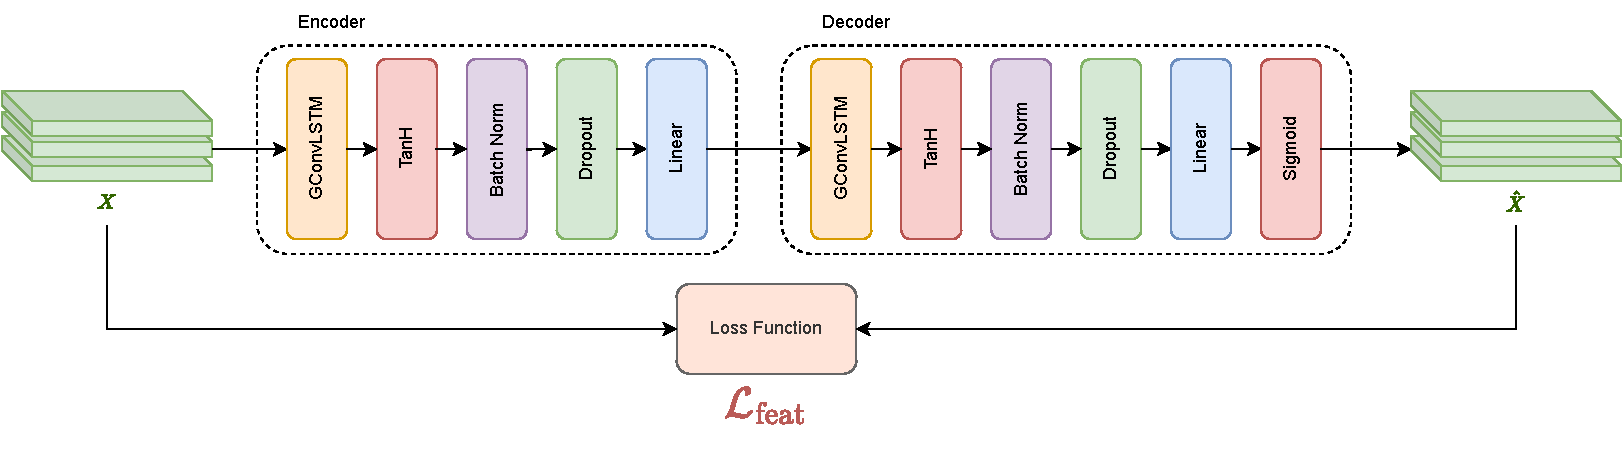
\includegraphics[width=0.9\textwidth]{./figures/Autoencoder.pdf}
\caption{Diagram representing the autoencoder as a combination of an encoder and a decoder.}
\label{fig:autoencoder}
\end{figure}


\todo[inline]{verify if this diagram is up-to-date}

The \gls{GConvLSTM} cell, as implemented by \cite{rozemberczki2021pytorch}, and initially proposed by \cite{Seo_2018}, is parameterized by the number of input channels $N_{\text{in}}$, the number of output channels $N_{\text{out}}$, and the size of the Chebyshev polynomial filter $K$. The cell executes graph-based convolutions on the input tensor $x$, with the knowledge of the graph edge's descriptor tensor \texttt{edge\_index}, to yield the hidden state $h$ and the cell state $c$. These states are then propagated through the sequence for subsequent iterations, defined by the $k$ discrete temporal segments of which the input $x$ is composed. This enables the model to capture and encode the temporal dynamics of the data.

\begin{equation}
    \text{GConvLSTM}: \mathbb{R}^{D_1 \times D_2 \times \ldots \times D_N \times N_{\text{in}}} \rightarrow \mathbb{R}^{D_1 \times D_2 \times \ldots \times D_N \times N_{\text{out}}}
\end{equation}

Furthermore, as implemented in this layer, the order of the Chebyshev filter plays a pivotal role, as it defines the range of neighborhood aggregation. Specifically, it dictates how and how many local neighborhoods are expanded around each node during the convolutional process. This, in turn, influences the gradient computation during backpropagation, affecting both the receptive field and the capacity of the model to capture and integrate multi-hop relational information.

In a regular \gls{LSTM} implementation, all internal variables are calculated based on the sigmoid of combinations of fully connected layers as highlighted in the equations:

$$
\begin{aligned}
i_t & =\sigma\left(\boxed{W_{x i} x_t} + \boxed{W_{h i} h_{t-1}} + w_{c i} \odot c_{t-1}+b_i\right), \\
f_t & =\sigma\left(\boxed{W_{x f} x_t} + \boxed{W_{h f} h_{t-1}} + w_{c f} \odot c_{t-1}+b_f\right), \\
c_t & =f_t \odot c_{t-1}+i_t \odot \tanh \left(\boxed{W_{x c} x_t}+\boxed{W_{h c} h_{t-1}}+b_c\right), \\
o_t & =\sigma\left(\boxed{W_{x o} x_t} + \boxed{W_{h o} h_{t-1}} + w_{c o} \odot c_t+b_o\right), \\
h_t & =o \odot \tanh \left(c_t\right),
\end{aligned}
$$

Generalizing the \gls{LSTM}, a model developed for time-series forecasting, for graph inputs requires the adjustment of these operations for something that can handle graph-data input. For the \gls{GConvLSTM}, the authors implemented the graph convolution operator $\ast_\mathcal{G}$ proposed by \cite{cnn_graph}, in which a graph signal $x \in \mathbb{R}^{n}$ with $n$ nodes is filtered by a non-parametric kernel $g_\theta$ composed of vectors of Fourier coefficients.

\begin{equation*}
y = g_\theta \ast_\mathcal{G} x
\end{equation*}

On this implementation, $\ast_\mathcal{G}$ is modeled with the normalized graph Laplacian decomposition $L=U \Lambda U^T$, which would imply a model's complexity of $\mathcal{O}(n^2)$. To make it more feasible, the authors propose a truncated expansion of $g_\theta$ using Chebyshev polynomials $T_k$ and truncated laplacian $\tilde{L}$. This reduces the complexity to $\mathcal{O}(|\epsilon|n)$, with $\epsilon$ number of edges of the graph.

\begin{equation*}
y = g_\theta \ast_\mathcal{G} x = \sum_{k=0}^{K-1}\theta_k T_k(\tilde{L})x
\end{equation*}

Finally, it's possible to define the \gls{GConvLSTM} model.

\begin{equation}
\begin{aligned}
i & =\sigma\left(W_{x i}\ast_\mathcal{G} x_t+W_{h i}\ast_\mathcal{G} h_{t-1}+w_{c i} \odot c_{t-1}+b_i\right), \\
f & =\sigma\left(W_{x f}\ast_\mathcal{G} x_t+W_{h f}\ast_\mathcal{G} h_{t-1}+w_{c f} \odot c_{t-1}+b_f\right), \\
c_t & =f_t \odot c_{t-1}+i_t \odot \tanh \left(W_{x c}\ast_\mathcal{G} x_t+W_{h c}\ast_\mathcal{G} h_{t-1}+b_c\right), \\
o & =\sigma\left(W_{x o}\ast_\mathcal{G} x_t+W_{h o} \ast_\mathcal{G}h_{t-1}+w_{c o} \odot c_t+b_o\right), \\
h_t & =o \odot \tanh \left(c_t\right),
\end{aligned}
\end{equation}

\subsection{Fine Tuning}

The autoencoder, the most computationally demanding part of the entire model, owes much of its complexity to the \gls{GConvLSTM} layers in both the encoder and decoder. These layers execute graph convolution operations, which can become computationally intensive for large graphs due to their quadratic complexity, $\mathcal{O}(n^2)$, where $n$ is the number of nodes in the graph.

We suggest a pragmatic two-step training approach for the feature extractor to handle the computational demand more effectively. Initially, we train the autoencoder using the available source data, which allows us to establish a solid initial data representation. Subsequently, we fine-tune this representation with the target data, adapting it to the specific characteristics of the target domain.

Moreover, this method results in a fixed feature extractor not tightly coupled to the overall model. This flexibility is particularly beneficial when considering the parameter definition of the latter parts of the model, meaning that we can then focus on training the Prediction Network without feeling the effects that the choice of the feature extractor's parameter has on the results.

\section{Domain Adaptation} \label{sec:domainadap}

As one of the main challenges of a transfer learning task, domain adaptation is the process of adapting a model trained on one or more source domains (where abundant data is available) to perform well on a different but related target domain (where data is limited or has other distribution characteristics). Various approaches can be taken to tackle this problem in the different contexts that appear during the development of the model.

We suggest using two domain adaptors for this model: parameter sharing and a \gls{GRL}. The parameter sharing, which would be applied during a fine-tuning process after a pre-training, makes sure to start the network, which matters, the one that predicts the target values with the suitable weights to make it possible for this network to work correctly despite the lack of data points.

The \gls{GRL}, on the other hand, aims to help the feature extractor to produce domain-invariant features, which will then be extremely useful for transferring knowledge between different domains by making the encoder less sensitive to the specific characteristics of the source domain, thereby enhancing its ability to perform well on the target one. It's to be placed just after the encoder block of the autoencoder and before the decoder.

The \gls{GRL} is also used as part of an adversarial training strategy performed by a domain discriminator or classifier that tries to distinguish source and target domains. Since the \gls{GRL} reverses the gradient sign and scales it during backpropagation, it encourages the model to generate features that try to ``fool'' the domain classifier, which raises the loss but enforces the encoder to generate features that are domain-agnostic.

For the Domain Discriminator, we model it as a sequence of three operations: firstly, we apply a global mean pool to the features' tensor, followed by a linear layer, and then the softmax function. This will yield the probabilities that the features come from each domain (in this case, we have only two: source and target). With these probabilities, it's then possible to calculate a loss measure using \gls{BCE} loss. Figure \ref{fig:DomainDiscriminator} shows how this would look like and at which points of the overall model both the \gls{GRL} and Domain Discriminator would be placed.

In the Domain Discriminator block, a sequence of operations is designed to process the graph features effectively. Initially, a Top-K Pooling operation is employed to reduce the node count over all the graphs, selecting the $K_\text{pool}$ nodes with the most significant features from the last temporal segment output of the encoder. This process is essential for maintaining a consistent input shape for subsequent layers, ensuring the discriminator can operate uniformly on graphs from varying domains. After pooling, the features undergo batch normalization and dropout. The following linear layer projects the normalized and subsampled features onto a latent space, which a sigmoid function then squeezes into the $[0, 1]$ interval.

This operation translates the latent representations into probabilities, indicating the likelihood of the graph belonging to the target or source domain. These probabilities form the basis for computing the Domain Adversarial Loss with the \gls{BCE} Loss function. Figure \ref{fig:DomainDiscriminator} illustrates the placement of the \gls{GRL} and the Domain Discriminator within the overall model structure.


\begin{figure}[!ht]
\noindent\hspace{0.5mm}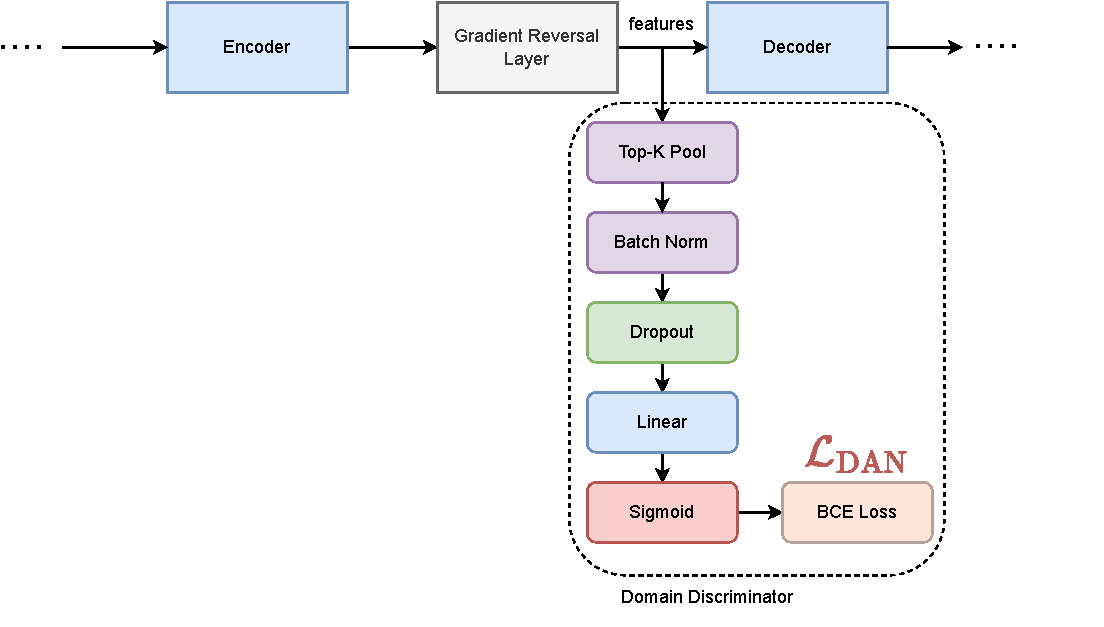
\includegraphics[width=0.9\textwidth]{./figures/DomainDiscriminator.pdf}
\caption{Diagram representing the architecture for the Domain Discriminator module.}
\label{fig:DomainDiscriminator}
\end{figure}


Given the output of the encoder block $H \in \mathbb{R}^{k\times N\times D_{lin}}$, with $k$ being the number of discrete temporal segments of which the input was composed, $N$ being the batched number of nodes of the input, and $D_{lin}$ the tunable dimension of the output of the linear layer of the encoder, we first select the last temporal segment from $H$. This choice is predicated on the understanding that the final snapshot encapsulates the most refined representation of the input graph, having undergone the full extent of recurrent processing through the \gls{LSTM} layers.

The next step in the pipeline is to apply the Top-K Pool to the graph. This is crucial in harmonizing node dimensionality across graphs from varied domains, which inherently may have disparate nodes. This step is essential to standardize the input size for the domain discriminator, allowing it to consistently and fairly assess the domain characteristics regardless of the original graph size. By retaining only the top $K_\text{pool}$ most significant nodes as per their learned representation in the encoder, Top-K Pooling concentrates on the most informative parts of the graphs, ensuring that the most critical structural and feature information is preserved for accurate domain discrimination.

\begin{equation}
	\text{Top-K Pool}:  \mathbb{R}^{N\times D_{lin}} \rightarrow \mathbb{R}^{K_\text{pool} \times D_{lin}}
\end{equation}

Following the dimensionality reduction via Top-K Pooling, the processed graph features are channeled through a linear layer, which projects the features onto a scalar. The subsequent application of the sigmoid function maps these projections to a $[0, 1]$ range, with the output values near 0 or 1 interpreted as the probability of the graph belonging to the target or source domain, respectively. These probabilities are then used to determine the Domain Adversarial Loss using the \gls{BCE} function - which will be presented and explained in Section \ref{ssec:bce}.

The general loss for the autoencoder training will then be defined accordingly to Equation \ref{eq:loss_ae}, with $\lambda$ being a tunable regularization parameter for balancing both the reconstruction loss $\mathcal{L}_{\text{feat}}$ and this adversarial loss $\mathcal{L}_{\text{DAN}}$.

\begin{equation} \label{eq:loss_ae}
	\mathcal{L}_{\text{AE}} = \mathcal{L}_{\text{feat}} + \lambda \cdot \mathcal{L}_{\text{DAN}}
\end{equation}


\section{Prediction Network} \label{sec:pred}

The second and final part of the model is the Prediction Network, which is responsible for making the next step prediction on the system state based on the features generated by the feature extractor and contextual timestamp features (time-of-the-day and day-of-the-week).


Given that the autoencoder developed is sufficiently good and can recreate the original input tensor $x$ with high accuracy, it's possible to consider that the encoder has appropriately learned how to extract the relevant features from the input. Based on that assumption, we extract the encoder from the trained autoencoder and use it as the feature extractor. Note that for feature extraction, we would only require the encoder block of the autoencoder, as the decoder and the domain discriminator blocks are only helpful tools for training the encoder.

Figure \ref{fig:Predictor} exposes the proposed architecture for the predictor block. It comprises an attention graph convolution block, an activation function, a linear layer, and a sigmoid normalization.

\begin{figure}[!ht]
\noindent\hspace{0.5mm}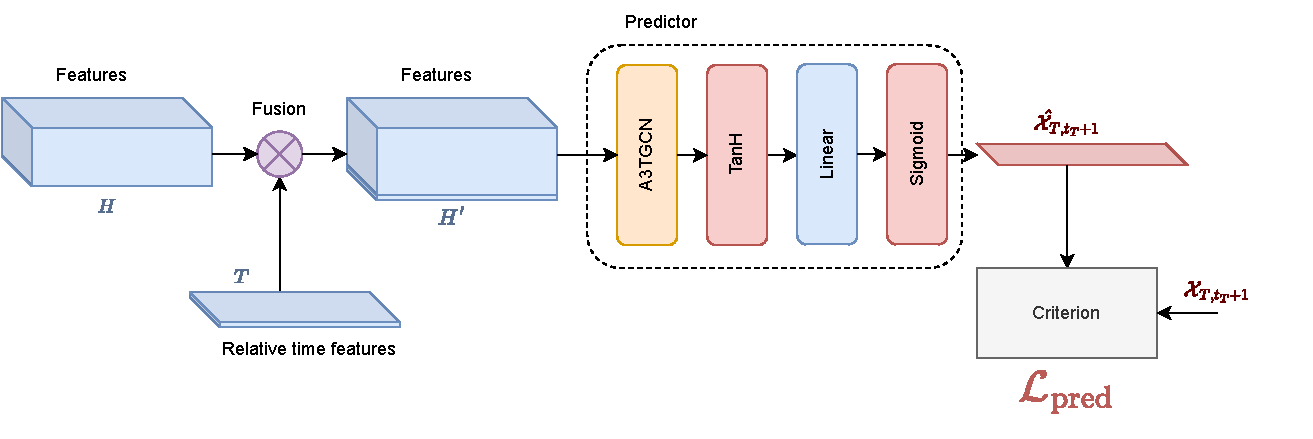
\includegraphics[width=0.9\textwidth]{./figures/Predictor.pdf}
\caption{Diagram representing the architecture for the Predictor network.}
\label{fig:Predictor}
\end{figure}

The tensor $H$ is the aforementioned output of the encoder block, while the tensor $T$ is the tensor that encapsulates periodic relative time features within our dataset. These features are derived from a sine-cosine transformation to exploit the inherent cycles in traffic flow, such as the daily rush hour peaks or the variation in traffic between weekdays and weekends. For the hour-of-the-day, we calculate:

\begin{equation}
\begin{aligned}
	hour\_sin=\sin\left(2\pi \cdot\frac{current\_hour}{hours\_in\_day} \right) & , & hour\_cos=\cos\left(2\pi \cdot\frac{current\_hour}{hours\_in\_day} \right)
\end{aligned}
\end{equation}

And for the day-of-the-week, we calculate:

\begin{equation}
\begin{aligned}
	day\_sin=\sin\left(2\pi \cdot\frac{current\_weekday}{days\_in\_week} \right) & , & day\_cos=\cos\left(2\pi \cdot\frac{current\_weekday}{days\_in\_week} \right)
\end{aligned}
\end{equation}

Concatenating these results, we create the tensor $T=[hour\_sin, hour\_cos, day\_sin, day\_cos]$, providing a continuous and differentiable representation of time. This tensor is fused with the regular \gls{ST} feature tensor, generating $H'$. For the fusion process, the tensor $T$ was extended (by repetition) to have all but the last dimension match the shape of $H$. The fusion technique applied to join them was a simple concatenation.

The leading actor of the Predictor block is the \gls{A3T-GCN} cell, proposed by \cite{abs-2006-11583} and implemented in the \textit{Pytorch Geometric Temporal} package \cite{rozemberczki2021pytorch}. It comprises two parts: first, a temporal convolution layer will generate $N_{t}$ hidden states $h$ for an input of $N_{t}$ temporal snapshots. These hidden states will then be the input of an attention model that will determine the context vector capable of understanding global variation trends, with which we can predict the system's future steps.



\section{Model Training} \label{sec:training}

After introducing all components of the model, it's opportune to explain, in detail, how exactly these components are supposed to be trained. Figure \ref{fig:training_script} shows the proposed training script for the whole model.

\begin{figure}[!ht]
\noindent\hspace{0.5mm}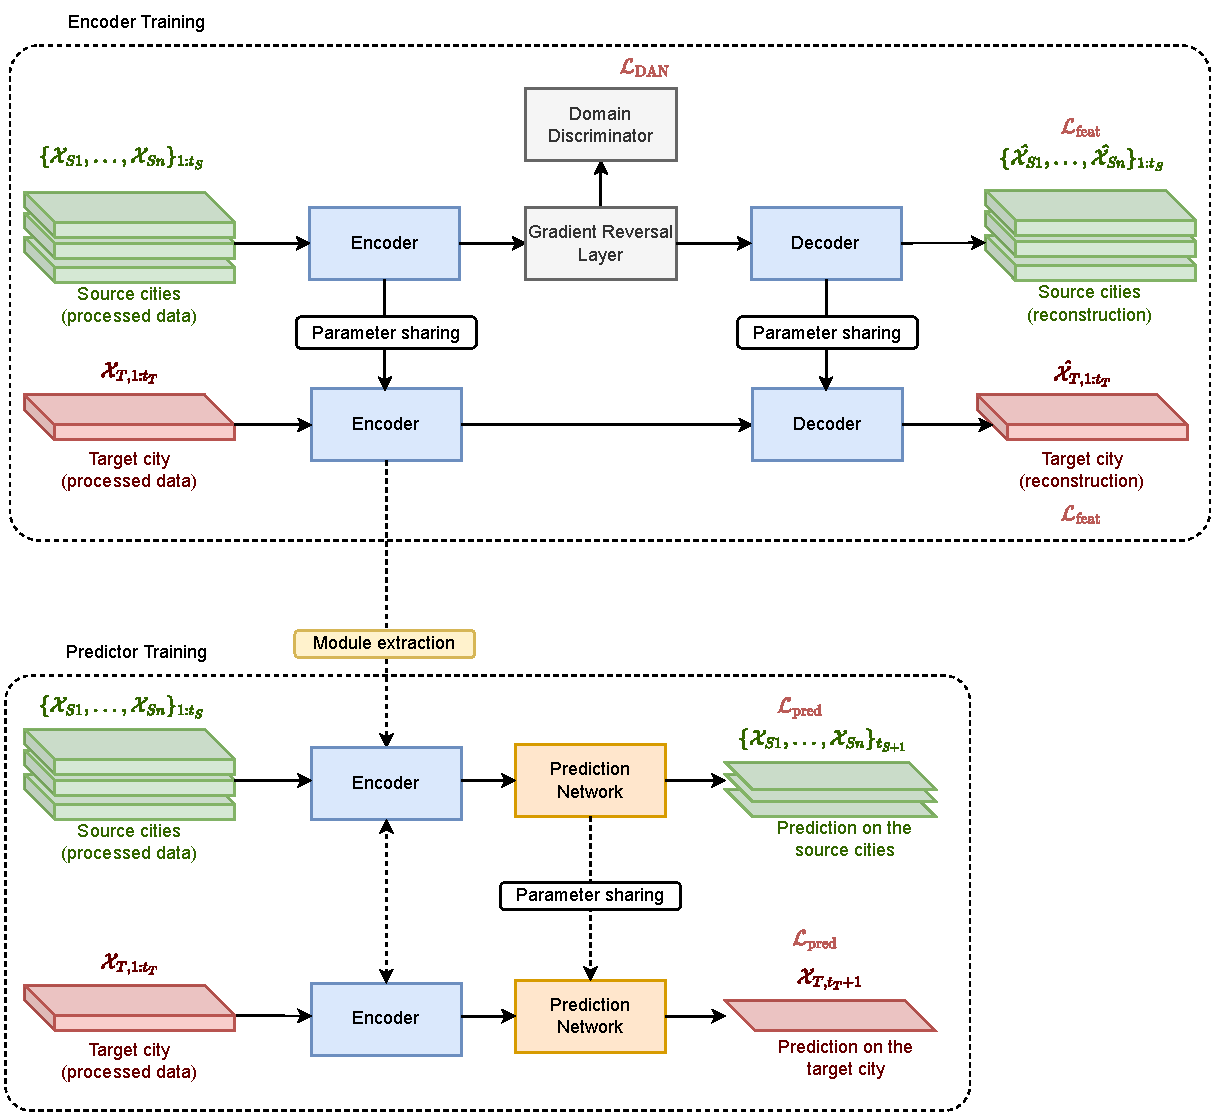
\includegraphics[width=0.9\textwidth]{./figures/training_script.pdf}
\caption{Diagram representing the training script and domain adaptation process.}
\label{fig:training_script}
\end{figure}

The training starts with pre-training the autoencoder and the domain discriminators using the source cities. As the decoder reconstructs the input, we can calculate a loss value composed of both a reconstruction criterion and an adversarial loss. After a determined number of epochs, the optimizer parameters are resettled, and the autoencoder is again trained with only the target city's data.

We freeze the autoencoder's weights for the second part and import the encoder block as the feature extractor. Again, the first step is to pre-train the predictor using the source cities' data and fine-tune it with the target city. For a more formal and structured explanation, Algorithm \ref{alg:ae} exposes the training process of the autoencoder with domain discriminator, while Algorithm \ref{alg:pred} does the same for the predictor block.

Since we use batch normalization as a regularization technique for all parts of our model, we selected \textproc{AdamW} \cite{abs-1711-05101}, a variation of \textproc{Adam}, as the optimizer algorithm. This makes sense because \textproc{AdamW} applies weight decay in a manner that is more compatible with batch normalization layers. Unlike the original \textproc{Adam} optimizer, which adjusts gradients directly and can undesirably impact batch normalization's scale and shift parameters, \textproc{AdamW} modifies the weights directly decoupled from the gradients, leading to more stable and consistent training dynamics.

Additionally, the utilization of \textproc{GradScaler} is noteworthy. This technique is employed to mitigate the underflow in gradient values during the backpropagation process, which occurs when the magnitudes of the gradients are so small that they are approximated to zero in the numerical precision being used. \textproc{GradScaler} addresses this issue by multiplying the loss value, from which gradients are derived, by a constant scaling factor. This operation increases the magnitudes of the gradients, preventing them from going to zero. After the backpropagation step, the gradients are then divided by the same scaling factor to restore their original magnitudes, preventing underflows without significantly impacting the performance.

Furthermore, it's interesting that we clarify the datasets used for each step of the training and evaluation of the model. During the pretraining phase, the autoencoder is trained on a combined dataset comprising both source and target data. This strategy facilitates the exposure of the domain discriminator to target features, which, in conjunction with the \gls{GRL}, orchestrates the adversarial training of the autoencoder. The datasets from the source domains are uniformly sized, while the smaller target domain dataset is iteratively cycled to align with the larger source datasets. Also, to make sure that the Domain Discriminator is trained in an unbiased way, for each \textproc{batch} from the dataloader, we randomly select one city and use only this selected city and the target city to train the \gls{DD}.

To enhance consistency, the pretraining of the predictor is also done on this same mixed dataset. The \textproc{optimizer\_params} for the different tasks are different and tuned based on the behavior of the loss of each task over the epochs, which are also task-specific parameters to be tuned depending on the learning capacity of each part of the model.

During the fine-tuning phase, we reset the optimizers using new, smaller learning rate and weight decay values and focused on the target dataset only. For the autoencoder, we still train both the \gls{GRL} and \gls{DD} to ensure that the model can adapt to the specific characteristics of the target domain while preserving the domain-invariant nature of the features. Since the fine-tuning dataset is smaller and the learning rate is reduced, we expect this to refine the model's performance on the target domain while maintaining its ability to generalize across domains. For this training phase, the target city dataset comprised, at a base case, 2 weeks' worth of data (meaning 3360 data points) extracted from the whole dataset via random split.

All testing on the predictor is done with a never-seen target data dataset. This dataset consisted of all non-used data of the target city. As in our setup, we had the same amount of data for all cities (6 months or 43\;200 data points). We used then ca. 40\;000 data points for the testing.

\begin{algorithm}
\caption{Autoencoder with Domain Discriminator Training Process }
\label{alg:ae}
\begin{algorithmic}[1]
\Require $AE\_params$, $DD\_params$, $num\_epochs$, $dataloaders$, $AE\_criterion$, $optimizer\_params$, $BATCH\_SIZE$, $lambda$
\Ensure Autoencoder $ae$, Domain Discriminator $dd$, Gradient Scaler $scaler$
\State \FunctionName{Encoder}, \FunctionName{Decoder} $ \gets$ \Call{Autoencoder}{$AE\_params$}
\State $dd \gets$ \Call{DomainDiscriminator}{$DD\_params$}
\State $scaler \gets$ \Call{GradScaler}{}
\State $optimizer \gets$ \Call{AdamW}{$\{ae, dd\}$, $optimizer\_params$}
\For{$epoch = 1$ \textbf{to} $num\_epochs$}
	\For{each $dataloader$ in $dataloaders$} \Comment{pre-training and fine-tuning dataloaders}
    \For{each $batch$ in $dataloader$}
        \State $total\_loss \gets 0$
        \For{each $data$ in $batch$}  \Comment{each batch can comprise $N$ different cities}
            \State $x, edge\_index, batch \gets data$
            \State $H \gets$ \Call{Encoder}{$x, edge\_index$}
	\State $H \gets$ \Call{GradientReversalLayer}{$H$}
            \State $dan\_loss \gets$ \Call{DomainDiscriminator}{$H, batch$}
            \State $x\_recons \gets$ \Call{Decoder}{$H, edge\_index$}
            \State $feat\_loss \gets AE\_criterion(x\_recons, x)$
            \State $loss \gets feat\_loss  + lambda \cdot dan\_loss$
            \State $total\_loss \gets total\_loss + loss$
        \EndFor
        \State \Call{Backward}{$scaler.scale(total\_loss)$}
        \State \Call{Step}{$optimizer$}
        \State \Call{Update}{$scaler$}
        \State $optimizer$.zero\_grad()
        \EndFor
    \EndFor
\EndFor
\end{algorithmic}
\end{algorithm}



\begin{algorithm}
\caption{Predictor Training Process}
\label{alg:pred}
\begin{algorithmic}[1]
\Require $PR\_params$, $num\_epochs$, $dataloaders$, $PR\_criterion$, $optimizer\_params$
\Ensure Predictor $pred$, Autoencoder $ae$
\State $pred \gets$ \Call{Predictor}{$PR\_params$}
\State  \FunctionName{Encoder} $ \gets$ \Call{Autoencoder}{\textit{pretrained}}\Comment{pre-trained and fine-tuned autoencoder}
\State $optimizer \gets$ \Call{AdamW}{$\{pred\}$, $optimizer\_params$}
\State $scaler \gets$ \Call{GradScaler}{}
\For{$epoch = 1$ \textbf{to} $num\_epochs$}
    \For{each $batch$ in $dataloaders$}
        \State $total\_loss \gets 0$
        \For{each $data$ in $batch$}
            \State $x, edge\_index, y, T\_features \gets data$
            \State $H \gets$ \Call{Encoder}{$x$, $edge\_index$}
            \State $H \gets$ \Call{FusionFeatures}{$H$, $T\_features$}
            \State $y\_hat \gets$ \Call{Predictor}{$H$, $edge\_index$, $batch$}
            \State $loss \gets$ \Call{PR\_Criterion}{$y$, $y\_hat$}
            \State $total\_loss \gets total\_loss + loss$
        \EndFor
        \State \Call{Backward}{$scaler.scale(total\_loss)$}
        \State \Call{Step}{$optimizer$}
        \State \Call{Update}{$scaler$}
        \State $optimizer$.zero\_grad()
    \EndFor
\EndFor
\Function{FusionFeatures}{$H$, $T$}
    \State $T \gets$ \Call{Extends}{$H$.shape}
    \State $H \gets H$ concatenated with $T$ along the feature dimension
    \State \Return $H$
\EndFunction
\end{algorithmic}
\end{algorithm}

\section{Loss Functions} \label{sec:loss_func}

In this Section, we define and explain the loss functions, also known as cost functions or criteria, that will be implemented or tested on the model or its parts. From the following criteria, \gls{MAE} and \gls{MAPE} are to be used exclusively as performance metrics. The purpose of listing and implementing a varied array of loss functions is to determine the best fit for our problem and data.

In this section, we define and elucidate the various loss functions, also recognized as cost functions or evaluation criteria, which are to be implemented or assessed within the model or its components. Among the specified criteria,\gls{MAE} and \gls{MAPE} will be exclusively utilized as performance metrics. Listing and implementing various loss functions is to determine the ones with the best training performance considering the problem and dataset.

\subsection{Mean Squared Error (MSE)}

As the most known and traditional loss function, \gls{MSE} is widely used in almost all fields of machine learning. In particular, it's one of traffic forecasting models' most ``standard'' loss functions as it focuses on minimizing significant errors.

\begin{equation}
\mathcal{L}(y, \hat{y}) = \frac{1}{N} \sum_{i=1}^{N} (y_i - \hat{y}_i)^2
\end{equation}


\subsection{Root Mean Squared Error (RMSE)}

A typical variation of the \gls{MSE}, \gls{RMSE} is widely used in almost all fields of machine learning for testing as a performance metric. It is based on the same concept that governs its base function but on the same scale as the input data. 

\begin{equation}
 \mathcal{L}(y, \hat{y}) = \frac{1}{N} \sqrt{\sum_{i=1}^{N} (y_i - \hat{y}_i)^2}
\end{equation}

\subsection{Mean Absolute Error (MAE)}

The \gls{MAE} is not supposed to be used as a criterion during the training phase, but rather, it's widely used as a performance metric for testing. It calculates the average absolute difference between the predicted and actual values. It treats all errors equally and is particularly robust when dealing with outliers.

\begin{equation}
\mathcal{L}(y, \hat{y}) = \frac{1}{N} \sum_{i=1}^{N} |y_i - \hat{y}_i|
\end{equation}

As it measures the average magnitude of errors in a set of predictions without considering their direction, the \gls{MAE} offers a scale-dependent interpretation of how far off the predictions are, on average, from the actual values.

\subsection{Mean Absolute Percentage Error (MAPE)}

Similarly, \gls{MAPE} is another performance metric to be applied during the testing phase. It uses the same logic as the \gls{MAE} but calculates the percentage error of the absolute difference between the predicted and actual values. It's used in the same context as MAE, but it's easier to interpret and practical when dealing with data represented in different scales.

\begin{equation}
\mathcal{L}(y, \hat{y}) = \frac{100\%}{N} \sum_{i=1}^{N} \left| \frac{y_i - \hat{y}_i}{y_i} \right|
\end{equation}

\subsection{Weighted Mean Squared Error (WMSE)}

As a variant of the MSE, the \gls{WMSE} amplifies the significance of errors in certain parts of the dataset by multiplying each error by a specific weight. It's helpful in scenarios where certain data points are more critical than others and should have more influence on the total loss. Mainly, it's applied to heavenly imbalanced datasets, as is the case for the data used in this work. This criterion is also known as Zero Inflation Loss when defining a weight for zero values.

\begin{equation}
\mathcal{L}(y, \hat{y}) = \frac{1}{N} \sum_{i=1}^{N} w \cdot (y_i - \hat{y}_i)^2
\end{equation}


\subsection{Mean Squared Logarithm Error (MSLE)}

This other variation of the MSE criterion consists of the mean of the squares of the logarithmic differences between the predicted and actual values. This criterion reduces the impact of significant errors on large true values. They are applied to problems where the target values have a wide range.

\begin{equation}
\mathcal{L}(y, \hat{y}) = \frac{1}{N} \sum_{i=1}^{N} (\log(y_i + 1) - \log(\hat{y}_i + 1))^2
\end{equation}

\subsection{Weighted Mean Squared Logarithm Error (WMSLE)}

The Weighted Mean Squared Logarithm Error (\gls{WMSLE}) is a sophisticated criterion that combines the aspects of the Mean Squared Logarithm Error (\gls{MSLE}) and the Weighted Mean Squared Error (\gls{WMSE}). It addresses the challenge of imbalanced datasets, focusing on penalizing the errors associated with non-zero targets more heavily.

This loss function is particularly adept at handling datasets where the prediction of non-zero values is more crucial than the prediction of zeros, which may be abundant but less informative. The \gls{WMSLE} is therefore especially useful when the cost of an error varies depending on the magnitude of the true value, such as in datasets with many zero entries but where accurate prediction of the non-zero values is paramount, which happens to be the case in our dataset (as discussed in Section \ref{sec:data_analysis}). The \gls{WMSLE} is defined as follows:

\begin{equation}
\mathcal{L}(y, \hat{y}) = \frac{1}{N} \sum_{i=1}^{N} w \cdot (\log(y_i + 1) - \log(\hat{y}_i + 1))^2
\end{equation}


\subsection{Custom Huber Loss}

The Custom Huber Loss combines the \gls{MSE} and \gls{MAE}. It's quadratic for small errors and linear for significant errors. We can also apply a Zero Inflation Loss for zero target values. It's advantageous when dealing with outliers and versatile as it can have the best of both criteria on the domains they are the best.

% Custom Huber Loss
\begin{equation}
\mathcal{L}_{\delta, w}(y, \hat{y}) = 
\begin{cases} 
\frac{1}{2} w \cdot (y_i - \hat{y}_i)^2 & \text{for } y =0, \\
\frac{1}{2} (y - \hat{y})^2 & \text{for } |y - \hat{y}| \leq \delta, \\
\delta \cdot (|y - \hat{y}| - \frac{1}{2} \delta) & \text{otherwise.}
\end{cases}
\end{equation}


\subsection{Log-Cosh Loss}

The Log-Cosh error is defined by the logarithm of the hyperbolic cosine of the difference between the prediction and actual values. It has a shape similar to the \gls{MSE} but is smoother and less sensitive to outliers. It's useful as it has the robustness of the \gls{MAE} while maintaining the smooth gradient of the \gls{MSE}. This loss function is differentiable, unlike \gls{MAE}.

% Log-Cosh Loss
\begin{equation}
\mathcal{L}(y, \hat{y}) = \frac{1}{N} \sum_{i=1}^{N} \log(\cosh(\hat{y}_i - y_i))
\end{equation}

\subsection{Binary Cross Entropy} \label{ssec:bce}

In the binary classification, the \gls{BCE} loss penalizes deviations from the actual labels by comparing the predicted probabilities against the ground truth, providing a robust gradient signal for model updates during training.

\begin{equation}
\mathcal{L}(y, \hat{y}) = -\frac{1}{N} \sum_{i=1}^{N} [y_{i} \log(\sigma(\hat{y}_{i})) + (1 - y_{i}) \log(1 - \sigma(\hat{y}_{i}))]
\end{equation}


\section{Baselines} \label{sec:baselines}

To better understand the performance achieved by the models elaborated, we propose using two different baselines: \gls{HA} and \gls{ARIMA}. In this Section, we explain each of the baselines, how they are calculated, and how they are applied to the dataset.

\subsection{Historical Average} \label{ssec:ha}

As one of the most common baselines in this field, \gls{HA} is based on the premise of temporal consistency, leveraging the average of data from corresponding time periods in the past—such as previous weeks—to forecast current traffic conditions.


\subsection{ARIMA} \label{ssec:arima}

As the other most famous and employed non-transfer baseline model, \gls{ARIMA} is a statistical time-series regression based on autoregressive (AR) and moving average (MA) components, which account for past values and errors, respectively, along with an integrated (I) element for differencing to induce stationarity \cite{1678242}.